\section{Parametric Curves (C3*2-16.3)}

The interpolating polynomials and splines that we have previously discussed can
only be used to interpolate functions. The techniques can be extended to
represent general curves in space that aren't necessarily functions, or even
curves which self-intersect. %The way we will do this is by ...

Suppose we wish to determine a polynomial or a pieceewise polynomial to connect
the points 

\[
(x_0, y_0), (x_1, y_1), \dots, (x_n, y_n) 
.\]

in the order given.

We can define a parameter $t$ with the interval $[t_0, t_n]$ with
\[
t_0 < t_1 < \dots < t_n
.\]

and construct approximation functions for $x$ and $y$ separately:
\[
x_i = x(t_i), \quad y_i = y(t_i)
.\]

\pagebreak
\Ex
\begin{center}
  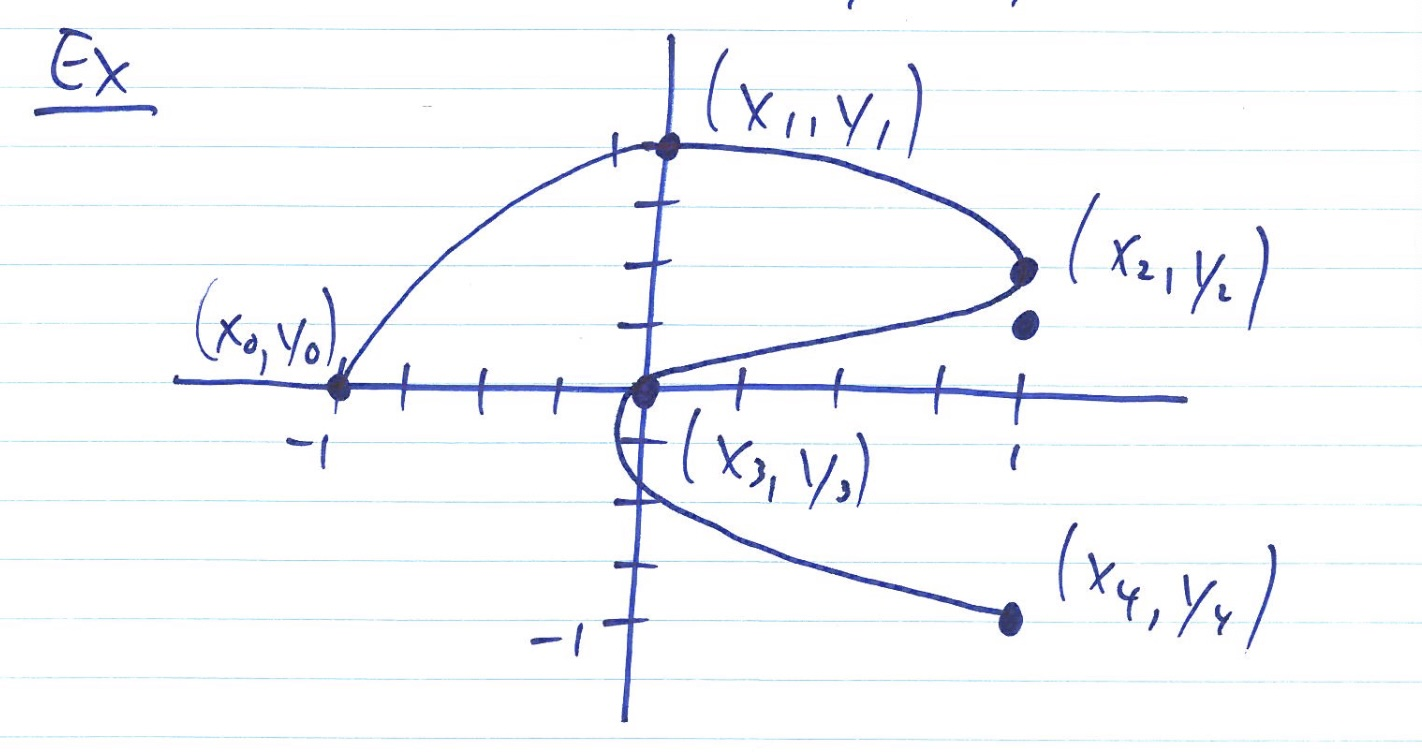
\includegraphics[width=0.8\textwidth]{./assets/parametric_curves_1.jpg}
\end{center}

There is flexibility in choosing the points $t_i$. Suppose we choose them to be
evenly spaced over $[0, 1]$. Then we can write

\[
\begin{array}{c|ccccc}
i & 0 & 1 & 2 & 3 & 4 \\ \hline
t_i & 0 & .25 & .5 & .75 & 1 \\
x_i & -1 & 0 & 1 & 0 & 1 \\
y_i & 0 & 1 & .5 & 0 & -1
\end{array}
\]

We could apply Lagrange interpolation for $x$ (or $y$) as a function of $t$.
The Lagrange Interpolating polynomials for $x$ and $y$ are

\[
x(t) = \left(\left(\left(64\,t - \frac{352}{3}\right)t + 60\right)t - \frac{1}{3}\right)t - 1
\]
\[
y(t) = \left(\left(\left(-\frac{64}{3}t + 48\right)t - \frac{116}{3}\right)t + 11\right)t
\] 

Alternatively, we could use a spline-based interpolation for $x$ and $y$.

Both of these approaches have the disadvantage that moving a single data point
affects the entire curve. We want the geometric property that changing one of
the points on the curve only changes one portion of the curve. \ie we want the
curve to only be affected locally by changes in the data.

\subsection{Piecewise Cubic Hermite Polynomials}
Because we want to avoid global changes, we might use a piecewise cubic Hermite
polynomial, which is just a spline with specific properties. We use one
polynomial for $x$ and one for $y$, both with respecto to $t$.

In other words, we specify the endpoints and the derivatives and the endpoints
to specify each portion of the curve. Thus, changin ga datapoint will only
change the two portions adjacent to the point, which means that smooth curves
can be easily and quickly modified.

\subsubsection{Uniqueness}

Quick answer: No.

\subsubsection{The Derivatives and Tangent Lines (C3*2-16.7)}
Suppose that the endpoints are at $t=0$ and $t=1$, then we only need to satisfy
the conditions on the quotients

\[
\frac{dy}{dx} (t=0) = \frac{y'(0)}{x'(0)}, \quad \frac{dy}{dx} (t=1)
= \frac{y'(1)}{x'(1)}
.\]

The actual values of $x'(0)$ and $y'(0)$ can be scaled by a common factor and
still satisfy these conditions. The larger the scaling factor, the closer the
curve comes to satisfying the tangent line near $(x(0), y(0))$.

A similar situation holds for 

\[
  (x(1), y(1))
.\]

\subsubsection{Guide Points (Cubic Bezier Curves)}
To simplify the process of specifying the slopes and to obtain a unique curve,
commercial software commonly specifies a second point called a
\enquote{guidepoint} which lies on the desired tangent line.

Suppose the endpoints are

\[
  (x(0), y(0)), \text{ and } (x(1), y(1))
.\]

and let the guidepoints be

\[
  (x_0 + \alpha_0, y_0 + \beta_0), \text{ and } (x_1 + \alpha_1, y_1 + \beta_1)
.\]

we will insist that $x$ satisfies

\begin{align*}
  x(0) &= x_0 & x'(0) &= \alpha_0 \\
  x(1) &= x_1 & x'(1) &= \alpha_1
\end{align*}

and that $y$ satisfies

\begin{align*}
  y(0) &= y_0 & y'(0) &= \beta_0 \\
  y(1) &= y_1 & y'(1) &= \beta_1
\end{align*}

Now there is a unique solution for $x$ and $y$:

\begin{align*}
    x(t) &= \left[ 2(x_0 - x_1) + (\alpha_0 + \alpha_1) \right] t^3 \\
         &\quad + \left[ 3(x_1 - x_0) - (\alpha_1 + 2\alpha_0) \right] t^2 \\
         &\quad + \alpha_0 t + x_0
\end{align*}

\begin{align*}
    y(t) &= \left[ 2(y_0 - y_1) + (\beta_0 + \beta_1) \right] t^3 \\
         &\quad + \left[ 3(y_1 - y_0) - (\beta_1 + 2\beta_0) \right] t^2 \\
         &\quad + \beta_0 t + y_0
\end{align*}

Popular graphics programs will typically use a slightly modified form for $x$
and $y$. They use B\'ezier polynomials which scale the derivatives $x'$ and $y'$
by a factor of $\mathbf{3}$ at the endpoints.

\begin{align*}
    x(t) &= \left[ 2(x_0 - x_1) + (\alpha_0 + \alpha_1) \right] t^3 \\
         &\quad + \left[ 3(x_1 - x_0) - (\alpha_1 + 2\alpha_0) \right] t^2 \\
         &\quad + \mathbf{3}\alpha_0 t + x_0
\end{align*}

\begin{align*}
    y(t) &= \left[ 2(y_0 - y_1) + (\beta_0 + \beta_1) \right] t^3 \\
         &\quad + \left[ 3(y_1 - y_0) - (\beta_1 + 2\beta_0) \right] t^2 \\
         &\quad + \mathbf{3}\beta_0 t + y_0
\end{align*}

\subsubsection{Fun Notes}

Generally, given that you don't have two points on the same point, i.e. you
don't have
$
  (x(0), y(0)) = (x(1), y(1))
$,
you can guarantee that the output curve will be continuous with a continuous
derivative. (i.e. $P \in C^1[a, b]$).

\section{Numerical Differentiation (C4*1-17.1)}

We also need to approximate the derivatives of functions. One approach is to
differentiate Lagrange polynomial approximations.

Suppose $x_0, x \in (a, b)$ and $f\in C^2[a,b]$.

Now

\begin{align*}
    f(x) &= P_{0,1}(x) + \frac{1}{2!} (x - x_0)(x - x_1) f''(\xi(x)) \\
         &= \frac{f(x_0)(x - x_1)}{x_0 - x_1} + \frac{f(x_1)(x - x_0)}{x_1 - x_0} 
         + \frac{(x - x_0)(x - x_1)}{2!} f''(\xi(x)) \\
         &\text{where } \xi(x) \in [a, b]
\end{align*}

Now differentiate:

\begin{align*}
    f'(x) &= \frac{f(x_1) - f(x_0)}{x_1 - x_0} + D_x \left[ \frac{(x - x_0)(x - x_1)}{2!} f''(\xi(x)) \right] \\
          &= \frac{f(x_1) - f(x_0)}{x_1 - x_0} + \frac{2 (x - x_0)(x - x_1)}{2} f''(\xi(x)) \\
          &\quad + \frac{(x - x_0)(x - x_1)}{2} D_x \left( f''(\xi(x)) \right)
\end{align*}

\subsection{More remarks}
Chapter 4 also considers numerical integration. We know how to integrate
polynomials, so we can just integrate the lagrange polynomial and call it a day.

